\documentclass[11pt]{article}
\usepackage[review]{acl}
\usepackage{times,latexsym}
\usepackage[T1]{fontenc}
\usepackage[utf8]{inputenc}
\usepackage{microtype,graphicx,booktabs,tabularx,array,amsmath,amssymb,xcolor,listings,xurl,needspace}
\newcommand{\todo}[1]{\textcolor{black!72}{\textbf{[TODO: #1]}}}
\newcommand{\code}[1]{\path{#1}}
\newcolumntype{Y}{>{\raggedright\arraybackslash}X}
\lstset{basicstyle=\small\ttfamily,breaklines=true,breakatwhitespace=false,columns=fullflexible,keepspaces=true,showstringspaces=false,frame=single,framerule=.25pt,framesep=5pt}
\title{From Prompt Semantics to Source Rankings in Generative Search}
\author{Anonymous ACL submission}
\begin{document}
\maketitle
\begin{abstract}
Requests about the same topic can ask for explanation, comparison, or immediate practical guidance. We study whether such differences in prompt meaning correspond to changes in source orderings in generative search. Our dataset contains 26,009 distinct prompt strings across 1,011 topics. We measure prompt semantics with external text embeddings and examine a direction from information seeking toward action readiness. Two answer generators use two strategies over frozen snapshots from two search engines. We distinguish sources ranked for relevance to a request from sources judged to support the answer actually produced, and separate source membership from ordering. Verified records establish the prompt population and partial execution coverage; a development example illustrates that an emitted source list can coexist with zero judged answer support. \todo{Insert verified findings and uncertainty for local stability, directional ranking changes, and relevance--support divergence, including condition-specific qualifications.} Population-level answers remain unverified. The study is descriptive: semantic associations do not establish why a model selected a source, and textual support does not establish internal source reliance.
\end{abstract}
\section{Introduction}
A request to explain the differences between two investment platforms and a request for instructions to transfer an account concern the same topic, but ask for different kinds of help. A source useful for the comparison may provide little evidence for the transfer procedure. In generative search, this distinction matters twice: when a system selects and orders sources, and when it produces an answer from the available evidence. An answer can list apparently relevant sources without those sources supporting the instructions that the answer gives.

We study how these source orderings vary with the meaning of the request. A \emph{prompt} is the user request supplied to the search-and-answer system. Its \emph{semantic space} is an external text-embedding representation in which nearby points are intended to describe similar meanings. One interpretable direction extends from seeking information toward requesting a decision or an action-enabling procedure. This direction is a measured property of prompt text, not a randomized treatment or a direct observation of a user's readiness to act.

The objects being compared also require care. A \emph{request-relevance ranking} orders supplied sources by how well they could help answer the request. An \emph{answer-support ranking} orders them by the importance of the answer content that their text supports. We obtain these assessments from judges with different inputs. The generator's own emitted ordering is a third observable, which does not by itself identify either relevance or support. In particular, a judge's finding that a source supports a statement is not evidence that the generator internally relied on that source.

These distinctions lead to two research questions:
\begin{enumerate}
\item \textbf{RQ1:} Do semantically similar prompts produce similar source orderings, and how do those orderings vary along interpretable semantic directions?
\item \textbf{RQ2:} How does this relationship differ between request-relevance rankings and answer-support rankings?
\end{enumerate}
We organize the investigation around \emph{local stability}, or agreement between orderings for nearby prompts; \emph{directional changes}, or systematic changes along a measured semantic coordinate; and \emph{relevance--support divergence}, or disagreement between the two judge-derived assessments. Models, engine snapshots, and search strategies are comparison conditions. They are not assumed to represent all language models or commercial search products.

The study uses a retained population of 26,009 synthetic requests associated with 1,011 keyword topics. Search is a deterministic local operation over frozen DuckDuckGo and SearxNG result snapshots. A prompt can nevertheless change the generated search queries, the evidence selected from those snapshots, and the sources available to the answer generator. Thus, two outputs are permutations of the same candidates only when the underlying evidence actually matches. The analysis separates membership changes from order changes rather than treating every pair of source lists as interchangeable permutations.

This paper makes three distinct contributions:
\begin{enumerate}
\item \textbf{A comparison framework.} We relate measured prompt semantics to source orderings while distinguishing evidence membership, generator-emitted lists, request relevance, and textual answer support.
\item \textbf{An auditable study resource.} We document prompt construction, semantic measurement, frozen retrieval, and execution units, including verified retained-population counts and gaps between intended and completed coverage.
\item \textbf{An empirical assessment with explicit scope.} We provide a real worked example and a source-by-source support procedure, and organize the empirical comparison around the two research questions. \todo{Replace this draft contribution's evidence-status clause with the substantive, qualified ranking findings once the matched analysis is verified.}
\end{enumerate}
The present draft reports verified descriptive checks and marks missing research results explicitly. It does not transfer the earlier manuscript's page-feature estimates or hidden-state findings to this experiment.

\section{Related Work}
\paragraph{Search intent and prompt meaning.}
Search requests have long been distinguished by what users seek to accomplish. Broder's taxonomy separates informational, navigational, and transactional search \citep{P006}. Our information-to-action direction is related to this concern with intent, but it is a continuous model-based description of text rather than a replacement for that taxonomy or a label of real user behavior. LLM2Vec provides a method for representing text with adapted language models \citep{P024}. Its general embedding results motivate a representation choice; they do not independently validate our readiness construct. We therefore keep the external encoder, its supervised semantic map, and the answer generator separate.

\paragraph{Language models as rankers.}
LLM-based reranking asks a model to order retrieved material for a request \citep{P041}. Our interest is the structure of variation across requests, rather than a claim of higher retrieval effectiveness. Fixed-pool reranking offers a direct comparison of permutations, whereas a search-and-answer pipeline may change the pool before producing an ordering. This distinction limits which observations in our agentic search records can answer an ordering-only question.

\paragraph{Visibility in generative search.}
Generative Engine Optimization studies how source content can change visibility in generated answers \citep{P044}. Content-centered benchmarks likewise examine source influence in generative search \citep{A002}. GEO includes comparisons of modified source content. Our focus is variation in prompt semantics and the distinction between request-relevant evidence and textual support for a completed answer. This places the request, rather than source-content optimization, at the center of the comparison.

\paragraph{Attribution, support, and reliance.}
Work on attribution evaluates whether generated statements can be supported by identified sources \citep{P072}; citation generation adds explicit references and evaluates their relationship to the answer \citep{P074}. ARES separates aspects of retrieval-augmented generation such as context relevance and answer faithfulness \citep{P083}. Our assessments also ask different questions, but support is graded here by the importance of the supported content within the answer. ContextCite studies attribution of model generation to context \citep{P068}, and \citet{A006} distinguish correctness from faithfulness in retrieval-augmented attribution. Matching source text to an answer is not an intervention on the generator and does not establish internal dependence. We use the narrower term \emph{textual answer support} throughout.

\section{Study Design and Methods}
\label{sec:methods}
\subsection{Overview and units of observation}
Figure~\ref{fig:overview} summarizes the implemented process. We first construct requests associated with a topic and a desired semantic destination, then measure the resulting text with frozen external embedding maps. For each execution condition, the generator formulates search queries and receives selected evidence from an immutable snapshot. It returns an answer and an ordered subset of evidence identifiers. Separate judgments assess relevance to the request and support for the completed answer.

A \emph{topic} is the dataset's keyword grouping, such as ``robinhood vs etrade.'' An \emph{information need} is the underlying question or practical objective a person wants to resolve; its count cannot be inferred from the number of topics. A \emph{prompt variant} is one retained request string associated with a topic. Variants may change purpose as well as wording, and have not been verified as meaning-preserving paraphrases of one base question. A \emph{search query} is an intermediate string generated for retrieval. An \emph{execution cell} is a prompt paired with a generator, engine snapshot, strategy, and recorded evidence condition. An \emph{answer} is the resulting text. A \emph{source} is an identified URL with the exact title and snippet text supplied as evidence, not a fetched full document. A \emph{judgment} is a separate evaluation of one cell or one source within it. These units have different denominators.

\begin{figure*}[t]
\centering
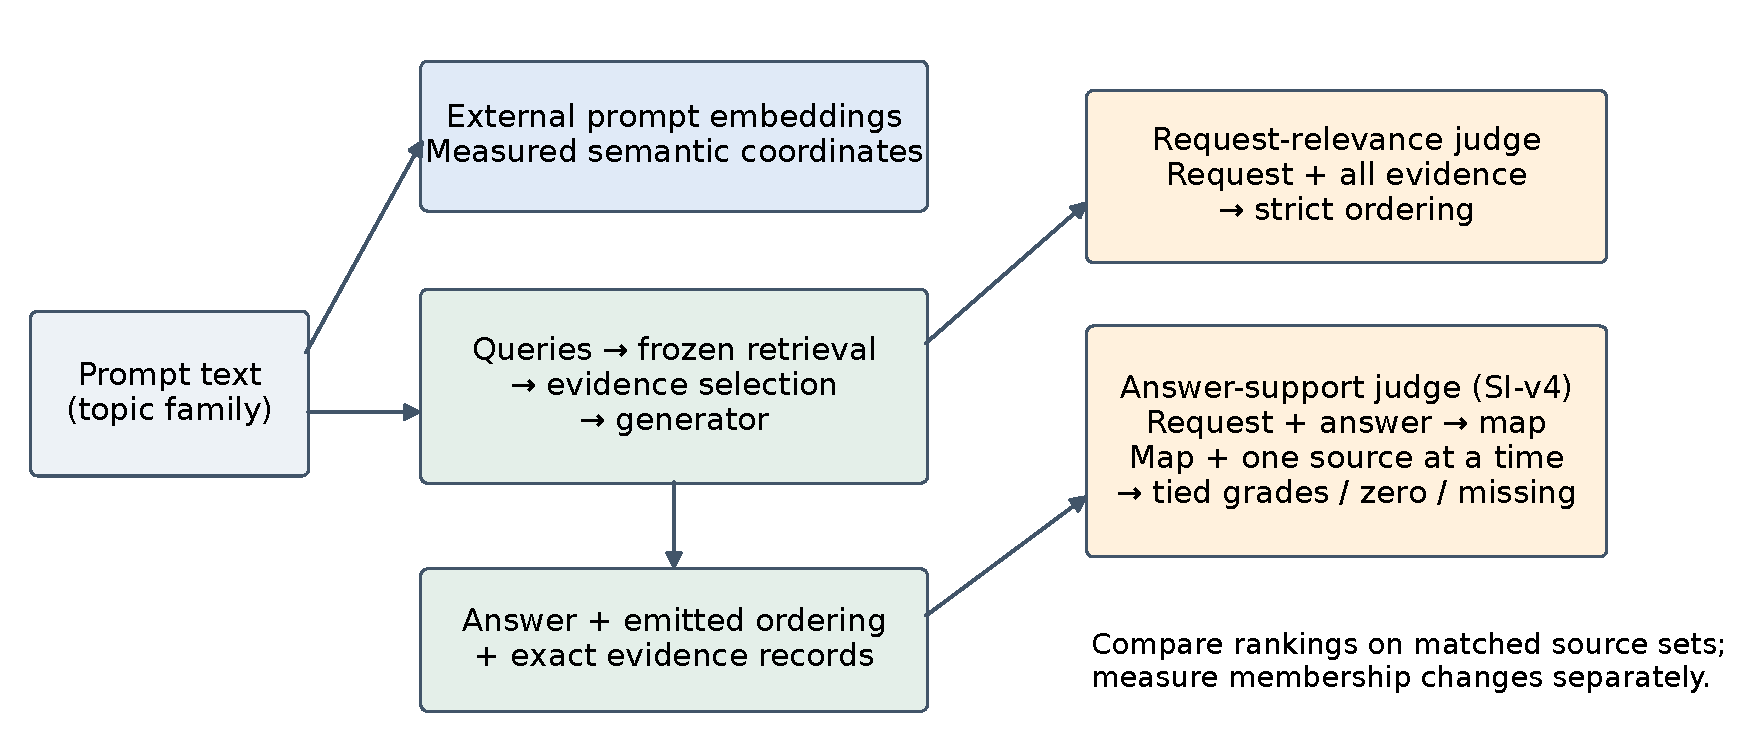
\includegraphics[width=\textwidth]{figures/study-overview.pdf}
\caption{Implemented measurement paths. Prompt embeddings describe request text; they are not hidden states of the answer generator. Local retrieval and evidence selection can change the source set across prompts. The relevance judge sees the request and all candidate evidence, but no answer. The support procedure first maps the completed answer without sources, then assesses each source separately. The diagram specifies inputs and outputs, not observed ranking effects or validation of the judgments.}
\label{fig:overview}
\end{figure*}

\subsection{A real running example}
\label{sec:example}
Table~\ref{tab:example} shows three actual prompts from one topic. We selected the illustrated execution by taking the lexicographically smallest natural-condition cell identifier in the saved 40-cell support-development audit, rather than selecting for a particular score. The other two prompts are retained variants from the same topic that illustrate different measured positions. This is a transparent illustration, not a representative sample of effects.

\begin{table*}[t]
\small
\begin{tabularx}{\textwidth}{@{}lYrrr@{}}
\toprule
 & Verbatim retained prompt & Intended & Measured & Measured\\
 & & target & axis 1 ($z$) & percentile\\
\midrule
A & What are the fundamental structural differences in how the platforms operate when looking at robinhood vs etrade? & .029 & $-1.688$ & .021\\[3pt]
B & I’m trying to transfer my investments this afternoon — what exact steps do I need to follow to set up a full transfer between robinhood vs etrade? & .924 & $-.329$ & .586\\[3pt]
C & Set up and verify same-day stock transfer from Robinhood to E*TRADE with account confirmation steps & .885 & .497 & .921\\
\bottomrule
\end{tabularx}
\caption{Real prompt-family illustration. The intended target is a construction instruction; the measured $z$ coordinate comes from the final aligned embedding maps; the percentile is the rank within the 26,009 retained strings. These are different scales. Only B's execution is inspected here: Llama, Reactive Loop, DuckDuckGo snapshot, natural evidence condition. Its saved generator ordering is Benzinga $\succ$ The Smart Investor $\succ$ Investopedia. All three historical SI-v3 support grades are zero. Request-relevance rankings, SI-v4 grades, and A/C execution comparisons remain \textbf{TODO}; no corresponding permutations are inferred.}
\label{tab:example}
\end{table*}

For prompt B, the generator was supplied with three snippets comparing the two platforms. The Benzinga snippet contrasts commission-free trades and a beginner-friendly app with research tools and a broader product range. The Smart Investor snippet contrasts ease of use with a more versatile trading environment; the Investopedia snippet also compares trading and resources. These snippets do not themselves present the transfer procedure requested. The saved generator list places Benzinga first, followed by The Smart Investor and Investopedia.

The answer begins: ``To set up a full transfer between Robinhood and E*TRADE, follow these steps: 1) Log in to your Robinhood account and go to the `Transfers' or `Account' section.'' It continues with a transfer procedure. This is quoted output, not verified financial guidance. The historical support judge assigned all three sources grade zero. Consequently there is no positive-support top source in this record, and top-source agreement with support is undefined. Treating the listed order as a support ordering, or arbitrarily putting the three zero-score sources into a strict bottom order, would create information that the judgment does not contain.

The example's intended target of .924 also differs from its measured percentile of .586. Percentiles and construction targets use different reference scales; this difference alone is not evidence of an acceptance failure. The illustration establishes the distinction between the measurements, not that more action-ready prompts generally have lower support. Appendix~\ref{app:example} records identifiers and provenance limits; Appendix~\ref{app:example-full} reproduces the answer and snippets. \todo{Complete this same example with verified relevance and SI-v4 outputs, and retrieve the corresponding executions for A and C without substituting illustrative rankings.}

\subsection{Dataset provenance and construction}
\label{sec:population}
The topic inventory contains 1,011 keyword groups. \todo{Recover the original keyword acquisition source, collection dates, licensing, language/domain composition, and mapping from topics to independently assessed information needs.} The earlier manuscript's dataset description is not sufficient provenance for the present retained population. A topic shared by requests for explanation and execution does not make those requests one independent question.

Prompt generation used Qwen3-32B and Gemma-4-31B-it with versioned instructions. The construction plan specified 30 semantic targets per topic, giving 30,330 topic--target slots, with four candidate proposals per generation task in the initial plan. The initial design used support-aware continuous targets, while later records contain axis-1 lattice targets and additional recovery rounds. We do not describe all rounds as one uniform grid. \todo{Reconcile the target-design chronology and per-round generation settings from their pinned manifests.}

The final text contract, \code{search-trigger-v2}, permits questions, imperative requests, and concise search phrases of 4--60 words on one normalized line. Topic metadata binds a candidate to its topic; the literal keyword string and standalone interpretation are optional. Generation instructions describe semantic destinations with verbal anchors, vary surface realization, and include feedback from earlier measured candidates. A recovery profile for high-axis targets asks for action-enabling requests without pretending that the search system has performed an action. Exact instructional templates and their dynamic substitutions appear in Appendix~\ref{app:templates}.

Quality checks combine mechanical text checks, independent model review, embedding measurements, and selection constraints. Under the final review contract, a candidate must be topical, express search intent, be web-answerable and natural, and receive at least 4/5 relevance. The strict selection check requires agreement with its target within .035 on normalized axis 1 under both frozen embedding views. Axis 2 is measured but is not that acceptance gate. Selection enforces one-to-one topic/target assignments and uniqueness of delexicalized templates, alongside a diversity gate. These are automated checks; they do not prove that all variants are distinct information needs or that people would issue them naturally.

The merged-candidate summary records 1,314,060 candidate records and 1,296,908 accepted records. The supporting summaries use different acceptance labels for the latter count, so we do not reconstruct a fine-grained filtering waterfall from them. The final files themselves contain 26,009 distinct strings and candidate identifiers, with exact text-hash joins to 26,009 measured-coordinate records. Qwen generated 13,515 retained strings and Gemma generated 12,494. Topics contain between 18 and 30 retained prompts. Table~\ref{tab:counts} distinguishes these direct file checks from manifest-level counts.

Retained-slot coverage is 26,009/30,330, or 85.75\%. It measures filled planned topic--target slots, not coverage of independent information needs, the web, or downstream executions. The saved selection summary leaves 4,321 slots unresolved. Its diversity gate passes, but its spacing gate and full-target-population verification do not. A passing final text-compliance audit must therefore not be described as a completely filled or evenly spaced design.

Prompt selection was iterative and used semantic feedback. \todo{Verify the provenance chronology needed to state whether any prompts, filtering thresholds, or semantic maps were tuned after inspecting downstream ranking results; absence of such tuning has not been established.} The final population is frozen for the executions described here, but freezing does not retrospectively establish independence from earlier development choices.

\begin{table*}[t]
\small
\begin{tabularx}{\textwidth}{@{}p{.28\textwidth}rY@{}}
\toprule
Unit or stage & Count & Evidence and interpretation\\
\midrule
Keyword topics & 1,011 & Counted in final prompt records; independent information needs unknown.\\
Planned topic--target slots & 30,330 & Construction manifest; 30 requested targets per topic.\\
Merged candidate records & 1,314,060 & Saved summary; raw merged archive not reread for this draft.\\
Accepted candidate records & 1,296,908 & Summary count; exact stage labels require reconciliation.\\
Retained prompt strings & 26,009 & Rehashed final file; all unique; 18--30 per topic.\\
Exact prompt--coordinate joins & 26,009 & Candidate IDs and UTF-8 text hashes verified.\\
Unresolved target slots & 4,321 & 14.25\% of intended slots; spacing gate did not pass.\\
\midrule
Full factorial target per generator & 312,108 & 26,009 prompts $\times$ 2 strategies $\times$ 2 engines $\times$ 3 recorded conditions.\\
Full target across two generators & 624,216 & Planned cells, not completed answers or support-judge calls.\\
Llama registry planned cells & 310,380 & Published registry; 1,728 fewer than full per-generator target.\\
Llama recorded completed / failed & 310,374 / 6 & Registry and bundle audit; payload rows not fully reread.\\
Qwen published completed cells & 24,218 & Audited JUPITER bundles only; not total cross-cluster completion.\\
Historical support-development cells & 40 & 40 prompts; 214 source tasks, two repetitions, SI-v3.\\
Final matched relevance/SI-v4 cells & \textbf{TODO} & No verified completed population export located.\\
\bottomrule
\end{tabularx}
\caption{Design and evidence counts. Prompt counts come from direct final-file checks; execution counts describe the publication audit at 2026-10-01 05:26:47 UTC, not live cluster state. Completed registry entries do not establish answer quality, usable rankings, or valid support judgments. The three historical evidence conditions are retained strata, not separate research questions. Per-model/engine/strategy completion and analysis-eligibility denominators remain to be verified.}
\label{tab:counts}
\end{table*}

\subsection{Measuring prompt semantics}
\label{sec:semantics}
We distinguish an \emph{intended destination}, supplied to prompt generation, from a \emph{measured position}, computed from the resulting text. The measurement uses two external LLM2Vec encoder views based on Qwen3-8B and Mistral-7B-Instruct-v0.2. It does not extract hidden states from the answer generator. Base-model revisions appear in Appendix~\ref{app:config}; exact encoder-adapter revisions still require a complete record.

The frozen map code normalizes each embedding and fits a ridge prediction of a model-consensus readiness label. It also fits rubric dimensions describing reversed information seeking, evaluation, selection commitment, and action implementation. A singular-value decomposition of their coefficient matrix supplies two supervised directions. The scalar predictor and the first supervised direction are related summaries, but they are not the same measurement. The aligned views yield the saved consensus axis-1 coordinate used in the worked example. The final map also reports a rank percentile within the retained population. This percentile preserves order but does not make semantic distances equally spaced or represent a probability of action.

A frozen calibration report contains 4,519 usable development items and 3,570 usable confirmation items. Scalar-prediction Spearman correlations with model-consensus labels are .680 for the Qwen view (saved 95\% interval [.661, .698]) and .732 for the Mistral view ([.717, .746]). The saved intervals use 1,000 bootstrap resamples of confirmation rows, with fixed predictions; they do not refit the encoders or account for dependence among related prompts. These are construct checks against model judgments, not validation against human intent or behavior. \todo{Verify encoder adapters, calibration-item provenance, label-judge identities, exclusion counts, and the consequences of related prompts for these row-resampled intervals.} Agreement between the two views in the selected population is additionally conditioned on selection that already required their agreement.

Figure~\ref{fig:geometry} characterizes the retained population without claiming a ranking result. A broader semantic-neighborhood analysis would compare distances between the external prompt embeddings; a one-dimensional coordinate can only characterize one direction within that space. The saved permutation-analysis code implements separate directional fits, and does not establish the full-space neighborhood relationship in RQ1.

\begin{figure*}[t]
\centering
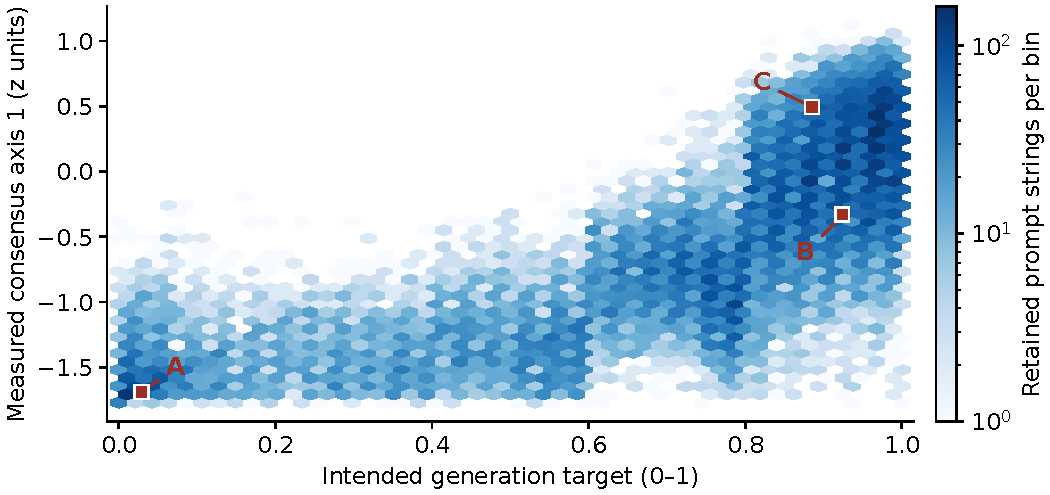
\includegraphics[width=.88\textwidth]{figures/target-measurement.pdf}
\caption{Construction targets and measured positions for all 26,009 retained prompt strings. Each hexagonal bin counts exact prompt--coordinate joins; color shows count on a logarithmic scale. The vertical coordinate is the final consensus axis-1 $z$ value, not a probability or a generator hidden state. A, B, and C identify the real variants in Table~\ref{tab:example}. This is a descriptive population census, so no sampling interval is drawn. It characterizes the selected population and the distinction between scales; it does not estimate semantic-to-ranking association or validate the intended target scale.}
\label{fig:geometry}
\end{figure*}

\subsection{Search, evidence selection, and generation}
\label{sec:generation}
The implemented engines are immutable snapshots of DuckDuckGo and SearxNG search results. For a generated query, the local adapter prioritizes exact keyword/query matches, then lexical overlap, stored engine position, a deterministic query--URL hash, and original row index. It returns at most 20 records per search action. A cross-encoder scores candidates for evidence selection. We use \emph{compaction} to mean this selection of a smaller evidence set; it must not be confused with silently shortening every snippet to a specified token count.

Parallel Expansion generates three distinct search queries, retrieves their results, deduplicates by URL, scores the combined records against the original request, and retains up to seven. Reactive Loop starts with search and permits up to three search actions. Each action retains up to three results scored against the current search query; accumulated observations are deduplicated by URL. The model may finish after observing evidence, or must finish when the action budget is exhausted. The distinct query used for compaction is part of the strategy difference. The pseudocode gives the conceptual procedure; Appendix~\ref{app:templates} contains the literal instructions.

\begin{figure}[t]
\small
\fbox{\begin{minipage}{.94\columnwidth}
\textbf{Parallel Expansion}\par
1. Generate three queries from the request.\par
2. Retrieve up to 20 records per query.\par
3. Merge records; deduplicate by URL.\par
4. Apply recorded evidence-condition hook.\par
5. Score against request; retain top seven.\par
6. Generate answer and evidence-ID ordering.\par\medskip
\textbf{Reactive Loop}\par
1. Start with no observations; require search.\par
2. For at most three search actions:\par
\hspace*{.6em}a. Generate query from request/observations.\par
\hspace*{.6em}b. Retrieve up to 20; apply condition.\par
\hspace*{.6em}c. Score against query; retain top three.\par
\hspace*{.6em}d. Accumulate deduplicated observations.\par
\hspace*{.6em}e. Allow finish after observing evidence.\par
3. Force finish when search budget is exhausted.\par
4. Return answer and evidence-ID ordering.
\end{minipage}}
\caption{Strategy pseudocode. Retrieval uses frozen snapshots. The condition hook records existing natural, ablated, or shuffled strata; those controls are not new research questions. Output validation and bounded repair are described in the text. Budgets count search actions and source records, not answer tokens.}
\label{fig:pseudocode}
\end{figure}

The answer generator sees the request and evidence records containing identifiers, URLs, titles, and snippets. It does not receive measured coordinates. Intermediate prompts expose accumulated observations, rather than a fetched full web page. The final output contains an answer and a ranking of supplied evidence identifiers, possibly a subset. The controller checks format and membership and records repair and truncation events. Its answer-length contract is 1,200 Python characters, separate from model output-token limits. Some support-preparation paths recover a longer answer from an exact matching trace when the stored answer is a truncated prefix. The analysis must therefore distinguish the answer stored for generation from the text actually judged. \todo{Report counts of repair, prefix recovery, truncation, unresolved source references, and exclusion by execution condition.}

The recorded generator families are Qwen3.8-27B and Llama-4-Scout-17B-16E-Instruct. The current Qwen bout configuration caps query output at 256 tokens and final output at 2,048 tokens; the inspected Llama adaptive configuration uses 256 and 4,096. Histories include budget changes, so these settings cannot be assigned to every historical cell. \todo{Join each execution to its pinned configuration, decoding settings, template hashes, and model revision before producing condition-level comparisons.} The cross-encoder is BAAI/bge-reranker-v2-m3; its pinned revision and documented settings appear in Appendix~\ref{app:config}.

The global snapshot is fixed, but candidate membership is \emph{not guaranteed fixed within a topic family}. Different generated queries can retrieve and select different records. An identical URL can also be paired with different evidence text. An ordering-only comparison requires matching source identity, title, text, and relevant presentation/configuration fields. Where pools differ, the records support a membership comparison and, separately, an ordering comparison on shared sources; the latter cannot describe excluded sources.

Historical natural, ablated, and shuffled conditions remain metadata strata. Their purpose and scope are documented with the configuration, but this manuscript asks no source-removal or input-order question. The shuffle hook precedes score-based compaction, so downstream sorting can undo a nominal shuffle. We do not interpret that label as proof that the generator received a different order. \todo{Audit effective presentation sequences and freeze which recorded strata enter each main comparison.}

\subsection{Obtaining relevance and answer-support orderings}
\label{sec:judges}
\paragraph{Request relevance.}
The implemented relevance judge receives the request and every evidence record supplied to that judging task, including URL, title, and snippet, but no generated answer. It must return each evidence identifier exactly once, from most to least useful for answering the request. This produces a strict judge-derived ordering. The schema calls it \code{ideal_relevance_ranking}; we use \emph{request relevance} because a judge output is not a verified ideal or human gold standard. The format cannot express ties and therefore imposes an order even when sources appear equally relevant. The Nemotron judging configuration identifies NVIDIA-Nemotron-3-Nano-30B-A3B-BF16. \todo{Verify completed relevance exports, exact per-run judge configuration, and an independent assessment of ranking quality.}

\paragraph{Textual support for the completed answer.}
A source can address the request without supporting the answer the generator chose to write. The current support-development procedure first constructs a source-blind map of the answer, then evaluates each source against that fixed map. The implementation is named \emph{Source Importance version 4} (SI-v4). Its purpose is to avoid conflating topical relevance, answer quality, and support for the answer as written.

In Stage A, the judge sees the request and the citation-masked complete answer, with indexed original word spans and no sources. It identifies assertions, recommendations, attributed reports, and claims about absence of information across the entire evidence set. It assigns each substantive claim an importance role within that answer: central, major, secondary, or peripheral. Every word must belong to a claim span or an explicit exclusion. Preserving words and accounting for spans are mechanical checks; neither proves that the map preserves meaning or importance.

In Stage B, the judge sees the same request and answer, the fixed map, and one unchanged source title/text record. It sees no source URL, other sources, generator identity, generator ordering, readiness value, or evidence-condition label. It identifies full or partial support, contradiction, or genuine uncertainty, with one to three representative source-passage witnesses per finding. The ordinal grade ranges from 0, no identifiable substantive support, to 5, support for most of the answer's essential content. Intermediate grades distinguish peripheral, secondary, substantial, and central supported content. The grade concerns importance \emph{within the completed answer}, including an off-target answer; it is not a relevance score, a fraction of claims, or a test of factual truth. Redundant sources may receive the same grade.

Uncertainty and map issues produce a missing grade, not zero. An unusable map blocks dependent scoring; a map flagged downstream prevents treating the cell as cleanly scored. Pure abstention and answers consisting only of global-absence claims can be ineligible for source-level scoring. One source cannot establish that information is absent from all sources. These cases require distinct denominators rather than being merged with unsupported but assessable answers.

Positive support grades form descending tied groups. Zero-grade sources are recorded separately and remain unranked in the positive-support ordering. Missing grades invalidate complete-cell metrics. When every score is zero, the positive top group is empty and top-source agreement is undefined; when grades are constant, a correlation needing grade variation is undefined. Grade zero must not be converted into missing data, and missing data must not be imputed as zero. The running example illustrates the all-zero case using historical SI-v3 judgments. It does not validate SI-v4.

\subsection{Semantic and ranking comparisons}
\label{sec:analysis}
The core descriptive question is whether prompts that are close in meaning have similar orderings when comparison is possible. We first distinguish equal evidence sets from unequal sets, then identify whose orderings are compared. A permutation comparison is meaningful only over specified candidates. The implemented agreement summaries include exact ordering agreement, first-source agreement, top-$k$ overlap, and Kendall agreement on sources common to both lists. The top-$k$ code uses the smaller of three and the two list lengths. Fewer than two common sources makes common-source Kendall agreement undefined. These summaries cannot turn source absence into a lower rank.

Let $p$ denote a request and $e(p)$ its unit-normalized external text embedding. Cosine distance, $1-e(p)^\top e(q)$, describes semantic separation of two requests $p$ and $q$ in that encoder view. Let $C(p)$ be the exact evidence records for a cell and $\pi(p)$ a specified ordering over those records. These symbols do not imply that the generator, relevance judge, and support judge share an ordering or that every support output is a strict permutation. \todo{Provide the verified local-neighborhood analysis, including encoder view, distance/neighbor rule, pool-matching criteria, overlap denominators, and eligible prompt-pair counts. No such population result is established by the saved directional fitter.}

For directional analysis, the existing exploratory implementation fits a regularized Bradley--Terry model within matched comparison strata. Each source has an intercept describing its baseline position and a slope describing how its relative preference changes with a measured semantic coordinate. Let $x$ be the measured coordinate standardized using training prompts within the fitted stratum. The utility of source $s$ is
\begin{equation}
 u_s(x)=\alpha_s+\beta_s x,
\label{eq:utility}
\end{equation}
and the fitted probability that $s$ precedes $t$ as
\begin{equation}
 \Pr(s\succ t\mid x)=\sigma\bigl(u_s(x)-u_t(x)\bigr),
\label{eq:bt}
\end{equation}
where $\sigma$ is the logistic function. This probability summarizes observed pairwise orderings under the model. A slope is not a causal effect of readiness or evidence of a model's internal ranking mechanism.

The fitter standardizes the axis using training prompts only and gives each task equal total weight across its observed source pairs. Missing candidates are not converted to pairwise losses. It compares the directional fit with an intercept-only baseline on held-out log loss, Brier score, and pairwise accuracy. Default settings require six distinct training questions and two test questions within a matched stratum, with ridge penalty 1. A deterministic text-hash split keeps identical text out of both partitions, but does not by itself separate semantically similar variants or independent information needs. Separate fits for separate coordinates do not amount to a joint model of the full semantic space.

Matched strata preserve exact evidence, configuration, presentation, and ranking-length requirements. The code separates fixed-pool direct reranking from agentic retrieval. Its reports carry \code{scientific_result=false}; no verified fixed-pool result was located for this draft. \todo{Supply the eligible-stratum inventory, fitted outputs, exclusion reasons, split assignments, and sample sizes before claiming directional ranking changes.}

Pooled metrics in the existing exploratory report are unweighted means over valid comparison rows, with a separate valid-row denominator for each metric. They are not automatically averages giving equal weight to every topic, model, or engine. Pair-weight normalization inside a fit is different from pooling across fits. The current fitter supplies no uncertainty intervals. \todo{Document the final pooling population, weights, dependency-aware uncertainty procedure, and direct comparisons across conditions; do not infer a difference merely because one estimate is significant and another is not.}

RQ2 requires relevance and support outputs joined to the same request, answer, and evidence. The existing support cell-metric function compares the \emph{generator} list with support grades; it is not already a relevance-versus-support analysis. Tied support can be compared with a strict relevance order using a tie-aware measure only when grades and candidate coverage make it defined. \todo{Verify the RQ2 join and specify each comparison's handling of positive grades, zero grades, ties, missing values, and all-zero cells. Report the unranked zero set separately from any full-vector rank correlation.}

\section{Results}
\label{sec:results}
\subsection{What the verified records establish}
The present evidence establishes a substantial retained prompt population and uneven completion coverage, rather than answers to both research questions. The final prompt and coordinate files contain 26,009 exact joins across 1,011 topics. Retained-slot coverage is 85.75\%, and only six topics have all 30 retained prompts. These are counts of frozen files, not sampled estimates, so confidence intervals would not describe uncertainty in those counts. Their relevance is that topic and target balance cannot be assumed when pooling later ranking summaries.

The publication audit records 310,374 completed Llama cells and six terminal failures against 310,380 registry entries. That registry is 1,728 entries smaller than the full 312,108-cell per-generator design. It also verifies 24,218 published Qwen completions in the inspected JUPITER bundles, without establishing total Qwen completion on HoreKa or later publication. Bundle manifests and object metadata were checked, but all row-level payloads were not reread. \todo{Resolve the Llama design/registry difference and report completed, valid-answer, valid-ranking, and matched-judge counts by generator, engine, strategy, and recorded condition.} Consequently, these numbers cannot establish balanced condition comparisons or a completed judgment corpus.

\subsection{RQ1: Local stability of source orderings}
\label{sec:local}
Do nearby prompts yield similar orderings? The available records do not yet supply a verified population estimate of this relationship. The pipeline establishes why the question must distinguish fixed evidence pools from changing source membership, and why a shared topic alone does not define a valid permutation comparison. It does not establish that local stability is high, low, or monotonic in embedding distance.

\todo{Insert the finding, its magnitude and uncertainty: eligible prompt-pair and family counts; semantic-distance ranges; exact/top-source agreement and common-source Kendall summaries; separate membership-overlap results; and missing/undefined denominators. Present the same measurements by generator, engine, and strategy, with a stated pooling rule. Add a main result figure only from the verified joined output.} Practical interpretation should express whether nearby prompts preserve the leading sources and how often observed changes instead arise because different evidence was available. Without these values, local semantic smoothness remains a question rather than a result.

\subsection{RQ1: Directional ranking changes}
\label{sec:directional}
Do orderings change systematically toward action-oriented requests? The verified population spans intended targets and measured coordinates, but Figure~\ref{fig:geometry} describes construction and measurement, not source-ranking behavior. The implemented directional fitter can compare a coordinate-dependent source-preference model with an intercept-only baseline; a fitted or tested improvement has not been verified for the present population.

\todo{Insert held-out differences in log loss, Brier score, and pair accuracy with uncertainty, valid-stratum counts, and interpretable changes in source-pair preference over observed coordinate ranges. Identify conditions with similar, weaker, or reversed patterns using direct condition comparisons. State whether a change survives exact-pool matching and distinguish full-space proximity from this one-dimensional result.} An improved directional prediction would show a descriptive association within eligible evidence/configuration strata. It would not show that changing a semantic coordinate while holding all other meaning fixed caused a rank change. Until matched results are available, no direction, effect size, or generality claim is warranted.

\subsection{RQ2: Relevance--support divergence}
\label{sec:divergence}
Does semantic structure differ between relevance and support rankings? The worked example verifies a narrower observation: one generator-emitted three-source list coexists with three zero historical support grades. Its positive-support top group is empty, so there is no defined top-source match to report. A relevance judgment for that same cell has not been verified. This is neither a population divergence rate nor a comparison of relevance with SI-v4.

In the 40-cell SI-v3 development audit, 209 of 214 source grades were identical across two repetitions (97.7\%), and 35 of 40 cells had identical complete grade vectors. A subsequent model-reference review identified semantic failures despite that repeatability. These diagnostics explain the motivation for separately mapping the answer in SI-v4; they do not constitute human validation, independent test accuracy, or evidence that SI-v4 resolves the failures. No completed SI-v4 population export is established here.

\todo{Insert matched relevance/SI-v4 findings: eligible cell count; defined tie-aware agreement and top-group overlap; proportions with zero support, all-zero vectors, uncertain grades, and unusable maps; uncertainty and differences by generator, engine, strategy, and semantic neighborhood or direction. Add independent judgment validation and distinguish development cases from held-out cases.} The interpretation must allow several possibilities: relevance can vary while supported content stays similar, support can vary because the answer changes, or both can change with the candidate set. The available evidence does not select among them.

\section{Discussion}
The value of comparing prompt semantics with source orderings depends on keeping three questions distinct: which sources were available, how they were ordered, and which parts of the answer they support. A change in an ordered list may be a retrieval-membership change rather than a change in preference among common candidates. A stable generator list may accompany a different answer and therefore different support judgments. These are observable distinctions that the study's records can support without a mechanism claim.

The information-to-action direction gives a readable interpretation to one part of prompt space. It does not exhaust semantic variation, and its model-based measurement does not make topic families collections of interchangeable paraphrases. In the example, explaining platform structure and requesting a transfer procedure involve different information needs. An association with their measured coordinates would describe variation in requests as constructed. It would not isolate a pure effect of wording or user readiness.

The strategy comparison has a concrete scope. Parallel Expansion selects evidence against the original request, whereas Reactive Loop selects each action's results against its current query and accumulates observations. Models and engine snapshots add further conditions. Any pooled finding must retain qualifications that arise from these differences. \todo{Add a discussion paragraph tied to the actual strongest and weakest verified conditions, including practical magnitude and uncertainty.} In the absence of those results, it would be premature to recommend a strategy or assert a stable pattern across the tested models.

Reliable data handling is necessary but does not validate interpretation. Frozen hashes can show which prompt and source text were used; schemas can ensure that identifiers are legal; word spans can establish that a quote is exact. None establishes whether a relevance ordering is sensible or a support grade is semantically correct. The historical repeatability result illustrates why a stable judge can still make stable mistakes. SI-v4's separate answer map makes those judgments more inspectable, but its validity remains an empirical question.

\section{Conclusion}
We study the relationship between measured prompt semantics and source orderings in generative search, separating local stability, directional changes, and relevance--support divergence. The verified record contains 26,009 prompt strings across 1,011 topics and an implemented pipeline with frozen retrieval and distinct judgment tasks. It also shows why intended prompt targets, measured text coordinates, generator-emitted orderings, and textual support cannot be treated as interchangeable measurements. \todo{State the principal verified ranking findings, magnitudes, and condition-specific qualifications when the matched analysis is available.} The present records do not yet establish population-level answers to the two research questions. Any eventual findings will be descriptive and conditional on the tested models, snapshots, strategies, evidence, and judges; textual support will still not establish internal source reliance.

\section*{Limitations}
\paragraph{Synthetic requests and unresolved independence.}
The prompts were generated and selected with model feedback. This limits generalization to naturally occurring requests and makes construction part of the observed distribution. Topics are not verified independent information needs, and exact-string deduplication does not remove semantic dependence. Treating all strings or all source pairs as independent would understate uncertainty. The keyword inventory's original provenance and domain balance also require completion.

\paragraph{Selection and semantic measurement.}
The retained set fills 85.75\% of planned target slots and fails the saved spacing criterion. Comparisons therefore concern the retained, selected population rather than a uniformly covered continuum. The two embedding views share model-derived supervision and selection constraints; high agreement does not validate human readiness. A percentile is population-relative and cannot support equal-distance interpretations. Missing adapter and calibration provenance limits exact reproduction until supplied.

\paragraph{Evidence and candidate membership.}
Frozen snapshots omit changes on the live web and represent snippets rather than complete pages. Conclusions concern the evidence shown, not everything a URL contains. Some historical support records aggregate passages, and the original generator traces were not included in the inspected support export; the final join must verify the exact evidence record rather than assuming a URL denotes one intact snippet. Generated queries and selection can change source membership; common-source comparisons then condition on an overlap that may be unrepresentative. Requiring exactly matched pools may leave few eligible families and narrow the population to which a permutation result applies.

\paragraph{Asymmetric judgments.}
Relevance sees URLs and all evidence together; support sees title/text for one source at a time and a completed answer. The tasks also differ in strict versus tied outputs. These differences can contribute to measured divergence independently of prompt semantics. Forced relevance orders conceal indifference, while zero-support and ineligible answers leave some support comparisons undefined. Independent semantic validation of both judges is missing, and development examples cannot serve as their own validation set.

\paragraph{Incomplete results and execution provenance.}
The snapshot of publication counts is not a current cross-cluster census, and the Llama registry differs from the full factorial target. Exact condition-level usable counts, configuration histories, and matched relevance/SI-v4 exports remain incomplete. The current exploratory report supplies no uncertainty intervals and no verified full-space neighborhood result. These gaps prevent substantive claims about the strength, direction, or consistency of the requested associations in this draft.

\paragraph{Interpretation and release.}
An answer may be supported by a source without the generator having used it internally, and support does not prove factual truth. Descriptive comparisons cannot resolve these mechanisms. The inspected source archives are private; no working anonymous release has been verified. We therefore make no claim that the full dataset or results are currently available to reviewers. \todo{Prepare and test an anonymous artifact link, verify redistribution rights for snapshot content, and document accessible files and exclusions.}

\bibliography{references}
\appendix
\clearpage
\onecolumn
\nolinenumbers
\section{Configuration and execution inventory}
\label{app:config}
This appendix records inspected settings, not a claim that a single configuration applies to every execution. Repository evidence was read at commit \code{9c92c93}; the manuscript handoff records the draft commit separately. Execution revisions must be read from each cell's manifest. The scientific output audit is dated 2026-10-01; no new inference was run to prepare this draft.

\begin{table}[!htbp]
\small
\begin{tabularx}{\textwidth}{@{}p{.20\textwidth}Yp{.34\textwidth}@{}}
\toprule
Role & Model identifier & Recorded revision\\
\midrule
Prompt construction & \code{Qwen/Qwen3-32B} & \path{9216db5781bf21249d130ec9da846c4624c16137}\\
Prompt construction / SI-v4 development & \code{google/gemma-4-31B-it} & \path{842da3794eaa0b77d5f08bae87a17459d91ff475}\\
Answer generator & \code{Qwen/Qwen3.8-27B} & \path{1d4bf0f2ff6012fd82039f2fa52739d0dd7c60c0}\\
Answer generator & \code{meta-llama/Llama-4-Scout-17B-16E-Instruct} & \path{92f3b1597a195b523d8d9e5700e57e4fbb8f20d3}\\
Relevance judge configuration & \code{nvidia/NVIDIA-Nemotron-3-Nano-30B-A3B-BF16} & \path{bf77c3174f68ad409e1c2aa60daeb46e32d1c606}\\
Evidence cross-encoder & \code{BAAI/bge-reranker-v2-m3} & \path{953dc6f6f85a1b2dbfca4c34a2796e7dde08d41e}\\
External encoder base & \code{Qwen/Qwen3-8B} & \path{b968826d9c46dd6066d109eabc6255188de91218}\\
External encoder base & \code{mistralai/Mistral-7B-Instruct-v0.2} & \path{63a8b081895390a26e140280378bc85ec8bce07a}\\
\bottomrule
\end{tabularx}
\caption{Identifiers found in construction records and inspected configuration/code. These roles must not be conflated: the Qwen prompt constructor, external encoder, and answer generator are different models. Base-encoder identifiers do not specify the full LLM2Vec adapters. Condition-level configuration joins and missing revisions remain explicit tasks; this table is not proof that every planned role has completed outputs.}
\label{tab:models}
\end{table}

\paragraph{Generation settings.}
The inspected Qwen bout settings use temperature 0, a master seed of 20260911 with cell-derived seeding, query/final output caps of 256/2,048 tokens, and disabled thinking. The inspected Llama adaptive settings use 256/4,096 output-token caps; its false thinking-disable flag does not mean thinking was forcibly disabled. Both strategies retain the separate 1,200-character answer contract. \todo{Record actual per-cell temperature, seed, context length, precision, tensor parallelism, runtime versions, and budget transitions from pinned manifests; reconcile repaired and trace-recovered answers.}

\paragraph{Support-development settings.}
The SI-v4 Gemma template specifies bfloat16 precision (BF16), tensor parallel size 4, concurrency 4, context length 73,728 tokens, temperature 0, disabled thinking, and semantic-task-derived seeds. Stage A and Stage B use 4,096 output-token caps and a maximum of two validation attempts. The recorded runtime is vLLM 0.28.0, Transformers 5.17.0, PyTorch 2.13.0, and XGrammar 0.2.7, on four A100-SXM4-40GB GPUs. These are prepared development settings, not a verified completed-run configuration. The full template accompanies this source in \code{appendices/si-v4-development-config.json}; its local tokenizer path remains an explicit deployment placeholder.

\paragraph{Snapshot and selection settings.}
The retrieval adapter's lexical term is four times query/keyword token overlap plus query/title-and-snippet overlap, followed by stored position and deterministic tie breakers. Both strategies retrieve at most 20 records per query and deduplicate by URL. \todo{Supply snapshot collection times, exact snapshot hashes, engine parameters, query language/locale, any upstream snippet truncation rule, and the executed cross-encoder input truncation settings.} Search count limits and final answer character limits do not specify encoder tokenization or upstream text truncation.

\paragraph{Exploratory fitter.}
The documented split seed is 20260916 and the content-hash modulus is 5. Axis standardization uses training data only; ridge penalty is 1; eligibility defaults require six training questions and two test questions. Matched evidence/configuration/presentation strata are required. These defaults must be checked against a saved report before any result is attributed to them. Current report metadata explicitly states that it is not a scientific result.

\section{Worked-example record and verification scope}
\label{app:example}
The illustrated cell is \code{14f3d6e1e67650a4eb97}, with prompt identifier \code{readiness-question:5f09b6606e92bc15e931c09b}. Its exact UTF-8 prompt hash is
\begin{quote}\small\path{acc90bb5cac32258f8264730e204da2bc792a8dfaa33b6d7fe120504cbe3498b}.\end{quote}
The saved audit uses the labels \code{llama4}, \code{Reactive-Snippet-Loop-v1}, \code{duckduckgo}, and \code{natural}. Selection by minimum natural-condition cell ID occurs within a development sample; it is not random sampling from all executions. The source export preserves saved-input integrity, but original generator traces were not included in that SI-v3 export. This limits independent verification of the original presentation sequence.

Exact snippets, the full answer, prompt variants, measured coordinates, and historical parsed outputs are included in \code{evidence/running-example.json}. Only the selected cell's task records are retained in that manuscript evidence file. Appendix~\ref{app:example-full} reproduces the answer and snippets for reading without a separate parser. All three grades refer to SI-v3. Request relevance and SI-v4 outputs are absent, and the manuscript does not replace them with invented values.

\section{Artifact inventory and outstanding evidence}
\label{app:artifacts}
The accompanying evidence inventory distinguishes direct file checks, published manifest audits, source-code behavior, and missing scientific outputs. The retained prompt file has SHA-256
\begin{quote}\small\path{1718321f8fc86f63d00aab30e87991ada9b62a59c5ef4ce99b5acef0df4d32e9},\end{quote}
and the final coordinate file has SHA-256
\begin{quote}\small\path{43189f68bcafc77f9dceb7a1a8d993251d4c2a739b401ef4fd24cb64e292682e}.\end{quote}
Both were read directly, joined by candidate identity, and checked against text hashes. The small population census and plot-bin counts accompany the draft. Full raw candidate archives and all execution payloads were not reanalyzed.

Before submission, essential evidence includes original topic provenance and independent-information-need mapping; reconciled construction chronology; exact execution/pool/configuration joins; condition-specific valid counts; validated relevance/SI-v4 records; local and directional ranking outputs with uncertainty; and a tested anonymous release with appropriate content permissions. These missing elements are not replaced by registry completion, calibration correlations, pilot repeatability, or the previous paper's results.

\clearpage
\section{Metric and denominator reference}
\label{app:metrics}
\begin{table}[!htbp]
\small
\begin{tabularx}{\textwidth}{@{}p{.24\textwidth}Yp{.26\textwidth}@{}}
\toprule
Measurement & Definition and interpretation & Denominator / undefined case\\
\midrule
Intended target & Normalized construction destination, 0--1; not an observed embedding. & Candidate generation task.\\
Measured axis 1 & Aligned, supervised embedding coordinate; final map stores consensus $z$. & Exact retained prompt text.\\
Population percentile & Axis-1 rank divided by $N-1$, for $N=26,009$. & Retained population; not a probability.\\
Retained-slot coverage & Selected prompts / planned topic--target slots. & 26,009 / 30,330.\\
Execution coverage & Validated completed cells / specified planned registry. & State generator, strata, and audit date.\\
Exact ordering agreement & Whether both specified ordered lists are identical. & Valid matched list pair.\\
Top-source agreement & Whether first sources agree; support top group needs separate handling. & Undefined if required top group is empty.\\
Top-$k$ overlap & Shared top-$k$ sources / $k$, $k=\min(3,|L_1|,|L_2|)$. & Empty list: no positive $k$.\\
Common-source Kendall & Relative ordering agreement restricted to shared source identities. & Fewer than two common sources: undefined.\\
Support grade & Ordinal 0--5; importance of supported content within an answer. & One eligible source--answer pair.\\
Positive support ordering & Descending tied groups for grades 1--5; zero set recorded separately. & Missing grade invalidates complete-cell summary.\\
Tie-aware agreement & Kendall $\tau_b$ accommodates grade ties for a specified comparison. & Constant side can make it undefined.\\
Held-out log loss/Brier & Prediction errors for observed ordered source pairs; smaller is better. & Eligible held-out pairs with within-task weights.\\
Pooled exploratory metric & Unweighted mean of valid report comparison rows. & Metric-specific valid-row count; not equal topic weight.\\
\bottomrule
\end{tabularx}
\caption{Terminology and metric reference. Existing generator-versus-support metrics must not be relabeled relevance-versus-support metrics. Missing observations, zero grades, and undefined statistics are distinct. Full-space neighborhood statistics, matched RQ2 exports, and uncertainty calculations remain to be supplied.}
\end{table}

\section{Full prompt templates and rendering details}
\label{app:templates}
The following blocks are instructional text extracted from the inspected implementation. Angle-bracket fields denote record-specific substitutions; braces in the population templates retain the renderer's variable names. They are not instructions to downstream judges to expose implementation metadata. Accompanying source excerpts preserve dynamic branches, evidence serialization, and schema builders. Exact per-execution rendered prompt and schema hashes must still be joined from original manifests. Historical template changes are not silently replaced by these current definitions.

\Needspace{8\baselineskip}
\subsection{Population generation and validation}
\lstinputlisting{appendices/population-generation.txt}
The readiness description interpolates adjacent anchors: understanding/explanation; investigating evidence or implications; evaluating alternatives; preparing a decision or plan; and requesting an immediate action-enabling step. An axis-1-only target leaves decision mode unconstrained. The renderer derives surface wording from the task seed and candidate slot. A high-axis recovery profile adds instructions favoring action-enabling language. The initial support-aware design also interpolates a decision-mode direction from comparing alternatives to implementation. Full branches, exact anchor strings, the earlier question-only contract, and high-axis instructions are retained in \code{appendices/population-renderers.py}; their generation-round use requires the provenance reconciliation in Section~\ref{sec:population}.
\lstinputlisting{appendices/population-validation.txt}
The independent validation prompt sees assigned topic metadata and candidate text. The answer generator's separate request does not automatically inherit that metadata. Hidden-context candidates therefore need an audit of what the executed request included; topic membership alone does not prove that the generator saw enough context.

\clearpage
\subsection{Search strategy templates}
\Needspace{12\baselineskip}
\medskip\noindent\textbf{Parallel query generation.}\par\smallskip
\lstinputlisting{appendices/parallel-query.txt}
\Needspace{12\baselineskip}
\medskip\noindent\textbf{Answer after parallel evidence selection.}\par\smallskip
\lstinputlisting{appendices/search-final.txt}
\Needspace{12\baselineskip}
\medskip\noindent\textbf{Reactive action.}\par\smallskip
\lstinputlisting{appendices/reactive.txt}
\Needspace{12\baselineskip}
\medskip\noindent\textbf{Forced finish after search budget.}\par\smallskip
\lstinputlisting{appendices/forced-finish.txt}
The evidence placeholder is a JSON array of records with \code{evidence_id}, \code{url}, \code{title}, and \code{text}, serialized with sorted keys and non-ASCII characters preserved. Identifiers such as S1 are local to the supplied evidence sequence, not global source names. The code supplies JSON response schemas and validates references after generation. Literal renderers and schema definitions accompany the source in \code{appendices/search-renderers.py}.

\Needspace{8\baselineskip}
\subsection{Request-relevance template}
\lstinputlisting{appendices/relevance.txt}
The evidence element is repeated for each candidate. The exact schema requires every evidence ID once. No answer is inserted. \code{appendices/relevance-renderer.py} retains dynamic rendering and schema source.

\Needspace{8\baselineskip}
\subsection{SI-v4 Stage A: source-blind answer map}
\lstinputlisting{appendices/si-v4-map.txt}
The shared suffix is:
\begin{lstlisting}
USER REQUEST:
<request>

ORIGINAL ANSWER UNITS:
[<answer_unit_id>] <original answer unit>
...

ANSWER WORD IDS:
[<word_id>] <original word>
...
\end{lstlisting}
Inputs use the configured citation-masking version while preserving the answer being evaluated. Word identifiers bind spans to the original answer; they do not authorize the judge to paraphrase or improve it. Dynamic schemas restrict fields and allowed identifiers. The schema builders and task rendering are retained in \code{appendices/si-v4-schemas.py}; a valid map is a prerequisite for dependent source tasks. \todo{Record the actual preprocessing version per judgment and its rendered-input hash in the final analysis export.}

\Needspace{8\baselineskip}
\subsection{SI-v4 Stage B: independent source support}
\lstinputlisting{appendices/si-v4-source.txt}
Stage B appends the same request/answer suffix, then:
\begin{lstlisting}
FIXED ANSWER MAP:
<validated answer map serialized as JSON>

SOURCE PASSAGES:
[<title_passage_id>] <unchanged title passage>
[<text_passage_id>] <unchanged source-text passage>
...
\end{lstlisting}
The source contains the entire supplied title/text record, partitioned into indexed passages. The prompt supplies neither its URL nor other sources. Representative witnesses locate support but are not a numerical scoring formula. Exact role, claim-kind, status, span, and grade constraints are defined in the accompanying schema excerpt. These templates document a development protocol, not verified accuracy or completed population judgments.

\clearpage
\section{Full answer and evidence for the running example}
\label{app:example-full}
The following answer is reproduced from the saved source-importance task. It is an experimental output, not financial advice or a verified procedure.
\begin{quote}
To set up a full transfer between Robinhood and E*TRADE, follow these steps: 1) Log in to your Robinhood account and go to the 'Transfers' or 'Account' section. 2) Initiate a transfer to an external account, selecting E*TRADE as the recipient. 3) Enter your E*TRADE account information. 4) Confirm the transfer details and submit. 5) Log in to your E*TRADE account to confirm the transfer. 6) If required, complete any additional paperwork or verification steps. Please note that specific steps may vary depending on individual circumstances. For detailed guidance, consult Robinhood and E*TRADE's official support resources.
\end{quote}
\begin{table}[!htbp]
\small
\begin{tabularx}{\textwidth}{@{}lp{.27\textwidth}Yr@{}}
\toprule
Generator rank & Title and source & Exact supplied snippet text & SI-v3 grade\\
\midrule
1 & Robinhood vs. E*TRADE • Which is Better for You? • Benzinga\newline \url{https://www.benzinga.com/money/robinhood-vs-etrade} & Robinhood offers commission-free trades and a user-friendly app for beginner investors, while E*TRADE provides more comprehensive research tools and a wider range of investment products for ... & 0\\[4pt]
2 & E*TRADE vs. Robinhood: Compare Brokerage Account Options\newline \url{https://thesmartinvestor.com/brokers/etrade-vs-robinhood/} & E*TRADE vs Robinhood : Compare Investing Features While Robinhood simplifies trading with a focus on cost-efficiency and ease of use, making it ideal for new investors, E*TRADE offers a more robust and versatile trading environment suitable for a broader range of investment strategies. & 0\\[4pt]
3 & Robinhood vs. E*TRADE - Investopedia\newline \url{https://www.investopedia.com/robinhood-vs-e-trade-4587955} & Robinhood offers commission-free trading but has cut corners to book profits while E*TRADE's competitive commissions allow customers to access an impressive basket of resources. & 0\\
\bottomrule
\end{tabularx}
\caption{Complete saved evidence for prompt B. Text, including the first snippet's trailing ellipsis, is copied from historical task input. Ranks are generator-emitted; grades are SI-v3 judge outputs, not human labels or SI-v4 results. The positive-support order is empty, the zero-grade set contains all three sources, and relevance remains unverified. Source URLs identify archived snippet records; current page contents were not used to replace them.}
\end{table}

\clearpage
\section{Reviewer-concern mapping for this draft}
\label{app:reviewer}
This editorial appendix maps supplied reviewer concerns to the revision. It is an author working aid and can be removed from the submission without removing scientific limitations or evidence placeholders.
\begin{table}[!htbp]
\small
\begin{tabularx}{\textwidth}{@{}p{.25\textwidth}Y@{}}
\toprule
Concern & Where addressed and what remains\\
\midrule
1. Readable abstract & Plain-language question, design, evidence boundary, and interpretation; under 200 words. Main findings remain explicit TODOs.\\
2. Clear introduction & Specific example, definitions, two research questions, and three distinct contributions. No priority or universal-model claim.\\
3. Methods before mathematics & Sections~\ref{sec:methods}--\ref{sec:judges} explain process, example, and judgments before Equations~\ref{eq:utility}--\ref{eq:bt}.\\
4. Complete dataset description & Section~\ref{sec:population} and Table~\ref{tab:counts} distinguish topics, strings, information needs, candidate stages, targets, and executions. Missing provenance and stage counts are marked.\\
5. Transparent setup & Sections~\ref{sec:generation}--\ref{sec:judges} and Appendices~\ref{app:config}, \ref{app:templates} specify inputs, models, budgets, characters versus tokens, filtering, and templates. Historical configuration joins remain TODOs.\\
6. Interpretable results & Section~\ref{sec:analysis} defines weighting and valid denominators. Section~\ref{sec:results} follows question, evidence, missing magnitude/uncertainty, condition differences, and interpretation.\\
7. Claims match evidence & Abstract, Results, Discussion, Conclusion, and Limitations distinguish semantic association, textual support, internal reliance, and development evidence.\\
8. Readable presentation & Distinct overview, population plot, design table, example, and strategy listing; captions below visuals; metric reference in Appendix~\ref{app:metrics}. Missing result plots are not fabricated.\\
9. Reproducibility and limitations & Appendices~\ref{app:config}--\ref{app:artifacts} document hashes, versions, and verification scope. Limitations follows Conclusion and explains consequences. Anonymous artifact access remains unverified.\\
\bottomrule
\end{tabularx}
\caption{Changes responding to the supplied editorial concerns. Original reviewer files were not available for separate inspection; this mapping addresses the supplied concerns without attributing additional claims to individual reviewers.}
\end{table}

\end{document}
